\section*{Цель}
Познакомиться с построением схемы заданной диаграммой Вейча.

\section*{Диаграмма Вейча}
\begin{figure}[H]
    \centering
    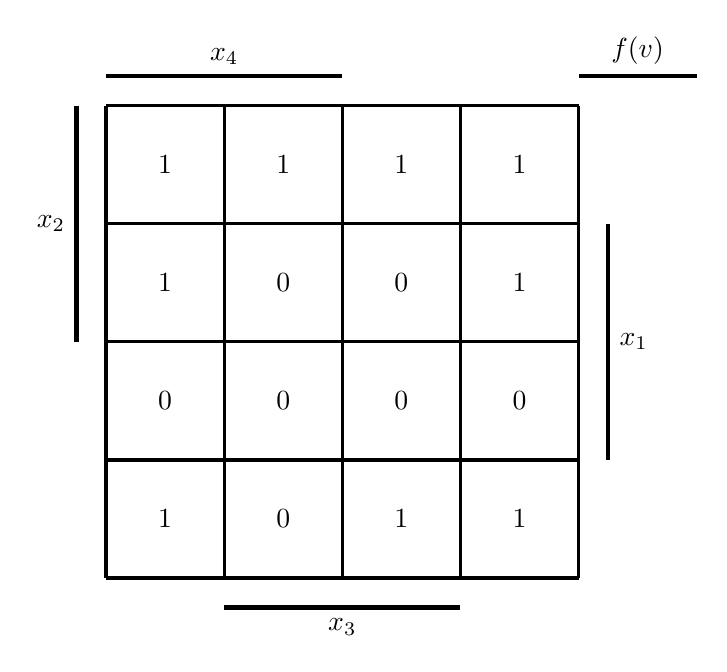
\begin{tikzpicture}[scale=1.5]
        % Рисуем сетку 4x4
        \draw[very thick] (0,0) grid (4,4);

        % Заполняем значениями (строка за строкой сверху вниз)
        % 1-я строка
        \node at (0.5, 3.5) {{1}}; \node at (1.5, 3.5) {{1}}; \node at (2.5, 3.5) {{1}}; \node at (3.5, 3.5) {{1}};
        % 2-я строка
        \node at (0.5, 2.5) {{1}}; \node at (1.5, 2.5) {{0}}; \node at (2.5, 2.5) {{0}}; \node at (3.5, 2.5) {{1}};
        % 3-я строка
        \node at (0.5, 1.5) {{0}}; \node at (1.5, 1.5) {{0}}; \node at (2.5, 1.5) {{0}}; \node at (3.5, 1.5) {{0}};
        % 4-я строка
        \node at (0.5, 0.5) {{1}}; \node at (1.5, 0.5) {{0}}; \node at (2.5, 0.5) {{1}}; \node at (3.5, 0.5) {{1}};

        % Рисуем внешние линии (метки переменных)
        % x4 сверху (над 1 и 2 колонками)
        \draw[ultra thick] (0, 4.25) -- (2, 4.25) node[midway, above] {$x_4$};
        % f(v) сверху (над 3 и 4 колонками)
        \draw[ultra thick] (4, 4.25) -- (5, 4.25) node[midway, above] {$f(v)$};
        
        % x2 слева (напротив 1 и 2 строк)
        \draw[ultra thick] (-0.25, 4) -- (-0.25, 2) node[midway, left] {$x_2$};
        
        % x1 справа (напротив 2 и 3 строк)
        \draw[ultra thick] (4.25, 3) -- (4.25, 1) node[midway, right] {$x_1$};
        
        % x3 снизу (под 2 и 3 колонками)
        \draw[ultra thick] (1, -0.25) -- (3, -0.25) node[midway, below] {$x_3$};

        % % Группа 1: Центральная строка нулей (4 ячейки)
        % \draw[blue, very thick, rounded corners=6pt] (0.1, 1.1) rectangle (3.9, 1.9);
        
        % % Группа 2: Квадрат 2x2 в центре сверху
        % \draw[red, very thick, rounded corners=8pt] (1.1, 1.1) rectangle (2.9, 2.9);
        
        % % Группа 3: Вертикальная пара в 2-й колонке снизу
        % \draw[green!60!black, very thick, rounded corners=4pt] (1.1, 0.1) rectangle (1.9, 1.9);
    
    \end{tikzpicture}
    \caption{Заданная диаграмма Вейча}
    \label{fig:veycha}
\end{figure}

\subsection*{ \boxed{\text{ Задание 1. }} }
\begin{quote}
    Найти МКНФ переключательной функции, заданной в виде диаграммы Вейча (\cref{fig:veycha}).
\end{quote}

Для нахождения МКНФ инвертируем диаграмму Вейча и выделим на ней один-клетки (\cref{fig:veycha_inv}):

\begin{figure}[H]
    \centering
    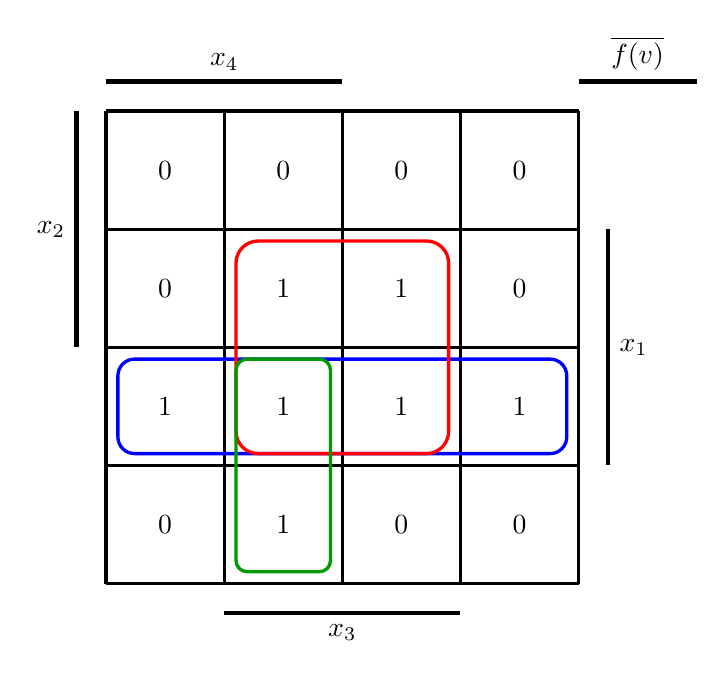
\begin{tikzpicture}[scale=1.5]
        % Рисуем сетку 4x4
        \draw[very thick] (0,0) grid (4,4);

        % Заполняем значениями (строка за строкой сверху вниз)
        % 1-я строка
        \node at (0.5, 3.5) {{0}}; \node at (1.5, 3.5) {{0}}; \node at (2.5, 3.5) {{0}}; \node at (3.5, 3.5) {{0}};
        % 2-я строка
        \node at (0.5, 2.5) {{0}}; \node at (1.5, 2.5) {{1}}; \node at (2.5, 2.5) {{1}}; \node at (3.5, 2.5) {{0}};
        % 3-я строка
        \node at (0.5, 1.5) {{1}}; \node at (1.5, 1.5) {{1}}; \node at (2.5, 1.5) {{1}}; \node at (3.5, 1.5) {{1}};
        % 4-я строка
        \node at (0.5, 0.5) {{0}}; \node at (1.5, 0.5) {{1}}; \node at (2.5, 0.5) {{0}}; \node at (3.5, 0.5) {{0}};

        % Рисуем внешние линии (метки переменных)
        % x4 сверху (над 1 и 2 колонками)
        \draw[ultra thick] (0, 4.25) -- (2, 4.25) node[midway, above] {$x_4$};
        % f(v) сверху (над 3 и 4 колонками)
        \draw[ultra thick] (4, 4.25) -- (5, 4.25) node[midway, above] {$\overline{f(v)}$};
        
        % x2 слева (напротив 1 и 2 строк)
        \draw[ultra thick] (-0.25, 4) -- (-0.25, 2) node[midway, left] {$x_2$};
        
        % x1 справа (напротив 2 и 3 строк)
        \draw[ultra thick] (4.25, 3) -- (4.25, 1) node[midway, right] {$x_1$};
        
        % x3 снизу (под 2 и 3 колонками)
        \draw[ultra thick] (1, -0.25) -- (3, -0.25) node[midway, below] {$x_3$};

        % Группа 1: Центральная строка нулей (4 ячейки)
        \draw[blue, very thick, rounded corners=6pt] (0.1, 1.1) rectangle (3.9, 1.9);
        
        % Группа 2: Квадрат 2x2 в центре сверху
        \draw[red, very thick, rounded corners=8pt] (1.1, 1.1) rectangle (2.9, 2.9);
        
        % Группа 3: Вертикальная пара в 2-й колонке снизу
        \draw[green!60!black, very thick, rounded corners=4pt] (1.1, 0.1) rectangle (1.9, 1.9);
    
    \end{tikzpicture}
    \caption{Инверсированная диаграмма Вейча}
    \label{fig:veycha_inv}
\end{figure}

Анализируя области, где функция равна $1$, получаем следующие дизъюнкты:
\begin{enumerate}
    \item \textit{\textcolor{blue}{Синяя область}}: Соответствует условию, где $x_1$, $\overline x_2$.
    \item \textit{\textcolor{red}{Красная область}}: Соответствует условию, где $x_1$, $x_3$.
    \item \textit{\textcolor{green!60!black}{Зеленая область}}: Соответствует условию, где $x_3$, $x_4$, $\overline x_2$.
\end{enumerate}

Таким образом:
\begin{equation}
    \overline{f(v)} = (x_1 \land \overline x_2) \lor (x_1 \land x_3) \lor (x_3 \land x_4 \land \overline x_2)
    \label{complex_iverted_f}
\end{equation}

Для упрощения визуального восприятия заменив $\land$ на $\cdot$ и найдем $f(v)$, используя законы де Моргана:
\begin{equation}
    f(v) = \overline{(x_1 \cdot \overline x_2) \lor (x_1 \cdot x_3) \lor (x_3 \cdot x_4 \cdot \overline x_2)}
\end{equation}
\begin{equation}
    \boxed{f(v) = (\overline x_1 \lor x_2) \cdot (\overline x_1 \lor \overline x_3) \cdot (\overline x_3 \lor \overline x_4 \lor x_2)}
\end{equation}

\subsection*{ \boxed{\text{ Задание 2. }} }
\begin{quote}
    Построить таблицу истинности найденной МКНФ. Входные переменные в таблице истинности расположить в порядке $x_1$, $x_2$, $x_3$, $x_4$. Входные состояния (строки таблицы истинности) расположить в порядке возрастания.
\end{quote}

\begin{table}[H]
    \centering
    \caption{Таблица истинности МКНФ}
    \label{table:truetable}

    \begin{tblr}[expand=\directlua]{
        colspec = { Q[c, m] Q[c, m] Q[c, m] Q[c, m] | Q[c, m] },
    }
        $x_1$ & $x_2$ & $x_3$ & $x_4$ & $f(v)$ \\
        \midrule
        $0$ & $0$ & $0$ & $0$ & $1$ \\
        $0$ & $0$ & $0$ & $1$ & $1$ \\
        $0$ & $0$ & $1$ & $0$ & $1$ \\
        $0$ & $0$ & $1$ & $1$ & $0$ \\
        $0$ & $1$ & $0$ & $0$ & $1$ \\
        $0$ & $1$ & $0$ & $1$ & $1$ \\
        $0$ & $1$ & $1$ & $0$ & $1$ \\
        $0$ & $1$ & $1$ & $1$ & $1$ \\
        $1$ & $0$ & $0$ & $0$ & $0$ \\
        $1$ & $0$ & $0$ & $1$ & $0$ \\
        $1$ & $0$ & $1$ & $0$ & $0$ \\
        $1$ & $0$ & $1$ & $1$ & $0$ \\
        $1$ & $1$ & $0$ & $0$ & $1$ \\
        $1$ & $1$ & $0$ & $1$ & $1$ \\
        $1$ & $1$ & $1$ & $0$ & $0$ \\
        $1$ & $1$ & $1$ & $1$ & $0$ \\
    \end{tblr}
\end{table}

\subsection*{ \boxed{\text{ Задание 3. }} }
\begin{quote}
    Собрать в графическом редакторе схему цифрового устройства, работа которого описывается найденной ранее МКНФ. Входные сигналы обозначить как $x_1$, $x_2$, $x_3$, $x_4$.
\end{quote}

\begin{figure}[H]
    \centering
    \includegraphics[width=1\textwidth]{figs/scheme.pdf}
    \caption{Схема цифрового устройства}
    \label{fig:scheme.pdf}
\end{figure}


\subsection*{ \boxed{\text{ Задание 4. }} }
\begin{quote}
    Показать результат работы компонента RTL Viewer для схемы, смоделированной в графическом редакторе.
\end{quote}

\begin{figure}[H]
    \centering
    \includegraphics[width=1\textwidth]{figs/RTL.pdf}
    \caption{RTL Viewer}
    \label{fig:RTL.pdf}
\end{figure}

\subsection*{ \boxed{\text{ Задание 5. }} }
\begin{quote}
    Смоделировать это же цифровое устройство в текстовом редакторе с помощью языка описания аппаратуры Verilog. Входные сигналы обозначить как $a_1$, $a_2$, $a_3$, $a_4$.
\end{quote}

\begin{listing}[H]
    \caption{Цифровое устройство на языке Verilog}
    \label{lst:verilogcode}
    \inputminted[
        % firstline      = 1,
        % lastline       = 10,
        % highlightlines = {1-10},
    ]{verilog}{code/verilog.v}
\end{listing}

\subsection*{ \boxed{\text{ Задание 6. }} }
\begin{quote}
    Показать результат работы компонента RTL Viewer для устройства, описанного с помощью языка Verilog.
\end{quote}

\begin{figure}[H]
    \centering
    \includegraphics[width=1\textwidth]{figs/RTL_verilog.pdf}
    \caption{RTL Viewer для Verilog}
    \label{fig:RTL_verilog.pdf}
\end{figure}

% ВАЖНО: в Quartus II такие действия, как отображение схемы в RTL Viewer, построение временных диаграмм и т. д., выполняются ТОЛЬКО ДЛЯ ФАЙЛА, ЗАНИМАЮЩЕГО НАИВЫСШЕЕ ПОЛОЖЕНИЕ В ИЕРАРХИИ ПРОЕКТА ИЛИ УПОМЯНУТОГО В ЭТОМ ФАЙЛЕ (его имя указано во вкладке Hierarchy окна Project Navigator, прямо под именем микросхемы)! Чтобы поместить на вершину данной иерархии другой файл, необходимо в том же окне Project Navigator открыть вкладку Files, выбрать нужный файл, щелкнуть по нему правой кнопкой мыши и выбрать Set as Top-Level Entity, после чего выполнить полную компиляцию проекта.

\subsection*{ \boxed{\text{ Задание 7. }} }
\begin{quote}
    Сравнить результаты работы компонента RTL Viewer для устройства, смоделированного в двух редакторах: графическом и текстовом.
\end{quote}

Визуальный осмотр \cref{fig:RTL_verilog.pdf} и \cref{fig:RTL.pdf} позволяет убедиться в идентичности RTL Viewer графической и текстовой схем.

Убедимся в этом, построив временные диаграммы (\cref{fig:sim_verilog.png,fig:sim.png}):

\begin{figure}[H]
    \centering
    \includegraphics[width=0.75\textwidth]{figs/sim_verilog.png}
    \caption{Временная диаграмма Verilog (без задержек)}
    \label{fig:sim_verilog.png}
\end{figure}

\begin{figure}[H]
    \centering
    \includegraphics[width=0.75\textwidth]{figs/sim.png}
    \caption{Временная диаграмма схемы (без задержек)}
    \label{fig:sim.png}
\end{figure}

Действительно, идентичность выходной функции $f$ на обоих диаграммах убеждает в тождественности графической схемы и Verilog кода. Подтверждает корректность вычислений таблица истинности (\cref{table:truetable}).

\subsection*{ \boxed{\text{ Задание 8. }} }
\begin{quote}
    Построить временные диаграммы при наличии и отсутствии задержек. Шаг сетки задать равным 30 нс. Время моделирования задать равным как минимум восьми шагам сетки. Входные сигналы задать в виде меандров с периодами, кратными 1-2-4-8 шагам сетки.
\end{quote}

Построим временную диаграмму с задержками на основе графической схемы (\cref{fig:sim_real.png}):

\begin{figure}[H]
    \centering
    \includegraphics[width=0.75\textwidth]{figs/sim_real.png}
    \caption{Временная диаграмма схемы (с задержками)}
    \label{fig:sim_real.png}
\end{figure}

Временная диаграмма без задержек представлена на \cref{fig:sim_verilog.png,fig:sim.png}.

\section*{Выводы}

В ходе данной лабораторной работы были освоены основы работы с диаграммой Вейча, языком Verilog в среде Quartus II.

Идентичность составленной графической схемы, алгоритма Verilog и таблицы истинности убеждают в корректности произведенных вычислений и построений.
